\documentclass{article}

\usepackage{tikz}
\usetikzlibrary{arrows.meta}

% ---------- Colors ----------
\definecolor{navy}{RGB}{20,55,100}
\definecolor{red}{RGB}{190,60,60}
\definecolor{redpale}{RGB}{255,235,235}
\definecolor{green}{RGB}{45,140,85}
\definecolor{greenpale}{RGB}{230,248,238}

\begin{document}
	
	\begin{figure}[ht]
		\centering
		
		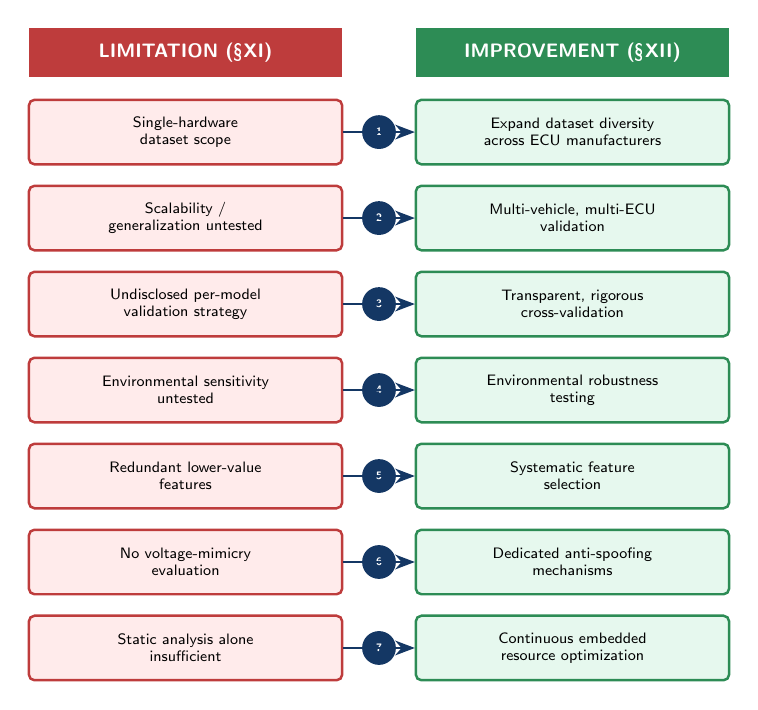
\begin{tikzpicture}[scale=0.78, transform shape]
			
			% ==========================================
			% HEADERS
			% ==========================================
			
			\node[
			rectangle,
			fill=red,
			text=white,
			minimum width=5.1cm,
			minimum height=0.8cm,
			align=center,
			font=\sffamily\bfseries\small
			] (h1) at (0,9.7)
			{LIMITATION (\S XI)};
			
			\node[
			rectangle,
			fill=green,
			text=white,
			minimum width=5.1cm,
			minimum height=0.8cm,
			align=center,
			font=\sffamily\bfseries\small
			] (h2) at (6.3,9.7)
			{IMPROVEMENT (\S XII)};
			
			
			% ==========================================
			% LIMITATION 1
			% ==========================================
			
			\node[
			rectangle,
			rounded corners=2pt,
			draw=red,
			fill=redpale,
			line width=0.9pt,
			minimum width=5.1cm,
			minimum height=1.05cm,
			align=center,
			font=\sffamily\scriptsize
			] (l1) at (0,8.4)
			{Single-hardware\\dataset scope};
			
			\node[
			rectangle,
			rounded corners=2pt,
			draw=green,
			fill=greenpale,
			line width=0.9pt,
			minimum width=5.1cm,
			minimum height=1.05cm,
			align=center,
			font=\sffamily\scriptsize
			] (i1) at (6.3,8.4)
			{Expand dataset diversity\\across ECU manufacturers};
			
			
			% ==========================================
			% LIMITATION 2
			% ==========================================
			
			\node[
			rectangle,
			rounded corners=2pt,
			draw=red,
			fill=redpale,
			line width=0.9pt,
			minimum width=5.1cm,
			minimum height=1.05cm,
			align=center,
			font=\sffamily\scriptsize
			] (l2) at (0,7.0)
			{Scalability /\\generalization untested};
			
			\node[
			rectangle,
			rounded corners=2pt,
			draw=green,
			fill=greenpale,
			line width=0.9pt,
			minimum width=5.1cm,
			minimum height=1.05cm,
			align=center,
			font=\sffamily\scriptsize
			] (i2) at (6.3,7.0)
			{Multi-vehicle, multi-ECU\\validation};
			
			
			% ==========================================
			% LIMITATION 3
			% ==========================================
			
			\node[
			rectangle,
			rounded corners=2pt,
			draw=red,
			fill=redpale,
			line width=0.9pt,
			minimum width=5.1cm,
			minimum height=1.05cm,
			align=center,
			font=\sffamily\scriptsize
			] (l3) at (0,5.6)
			{Undisclosed per-model\\validation strategy};
			
			\node[
			rectangle,
			rounded corners=2pt,
			draw=green,
			fill=greenpale,
			line width=0.9pt,
			minimum width=5.1cm,
			minimum height=1.05cm,
			align=center,
			font=\sffamily\scriptsize
			] (i3) at (6.3,5.6)
			{Transparent, rigorous\\cross-validation};
			
			
			% ==========================================
			% LIMITATION 4
			% ==========================================
			
			\node[
			rectangle,
			rounded corners=2pt,
			draw=red,
			fill=redpale,
			line width=0.9pt,
			minimum width=5.1cm,
			minimum height=1.05cm,
			align=center,
			font=\sffamily\scriptsize
			] (l4) at (0,4.2)
			{Environmental sensitivity\\untested};
			
			\node[
			rectangle,
			rounded corners=2pt,
			draw=green,
			fill=greenpale,
			line width=0.9pt,
			minimum width=5.1cm,
			minimum height=1.05cm,
			align=center,
			font=\sffamily\scriptsize
			] (i4) at (6.3,4.2)
			{Environmental robustness\\testing};
			
			
			% ==========================================
			% LIMITATION 5
			% ==========================================
			
			\node[
			rectangle,
			rounded corners=2pt,
			draw=red,
			fill=redpale,
			line width=0.9pt,
			minimum width=5.1cm,
			minimum height=1.05cm,
			align=center,
			font=\sffamily\scriptsize
			] (l5) at (0,2.8)
			{Redundant lower-value\\features};
			
			\node[
			rectangle,
			rounded corners=2pt,
			draw=green,
			fill=greenpale,
			line width=0.9pt,
			minimum width=5.1cm,
			minimum height=1.05cm,
			align=center,
			font=\sffamily\scriptsize
			] (i5) at (6.3,2.8)
			{Systematic feature\\selection};
			
			
			% ==========================================
			% LIMITATION 6
			% ==========================================
			
			\node[
			rectangle,
			rounded corners=2pt,
			draw=red,
			fill=redpale,
			line width=0.9pt,
			minimum width=5.1cm,
			minimum height=1.05cm,
			align=center,
			font=\sffamily\scriptsize
			] (l6) at (0,1.4)
			{No voltage-mimicry\\evaluation};
			
			\node[
			rectangle,
			rounded corners=2pt,
			draw=green,
			fill=greenpale,
			line width=0.9pt,
			minimum width=5.1cm,
			minimum height=1.05cm,
			align=center,
			font=\sffamily\scriptsize
			] (i6) at (6.3,1.4)
			{Dedicated anti-spoofing\\mechanisms};
			
			
			% ==========================================
			% LIMITATION 7
			% ==========================================
			
			\node[
			rectangle,
			rounded corners=2pt,
			draw=red,
			fill=redpale,
			line width=0.9pt,
			minimum width=5.1cm,
			minimum height=1.05cm,
			align=center,
			font=\sffamily\scriptsize
			] (l7) at (0,0.0)
			{Static analysis alone\\insufficient};
			
			\node[
			rectangle,
			rounded corners=2pt,
			draw=green,
			fill=greenpale,
			line width=0.9pt,
			minimum width=5.1cm,
			minimum height=1.05cm,
			align=center,
			font=\sffamily\scriptsize
			] (i7) at (6.3,0.0)
			{Continuous embedded\\resource optimization};
			
			
			% ==========================================
			% NUMBER CIRCLES
			% ==========================================
			
			\foreach \i/\y in {
				1/8.4,
				2/7.0,
				3/5.6,
				4/4.2,
				5/2.8,
				6/1.4,
				7/0.0
			}
			{
				\node[
				circle,
				fill=navy,
				text=white,
				font=\sffamily\bfseries\tiny,
				minimum size=0.55cm
				] at (3.15,\y) {\i};
			}
			
			
			% ==========================================
			% ARROWS
			% ==========================================
			
			\draw[
			-{Stealth[length=2.5mm]},
			draw=navy,
			line width=0.9pt
			] (l1.east) -- (i1.west);
			
			\draw[
			-{Stealth[length=2.5mm]},
			draw=navy,
			line width=0.9pt
			] (l2.east) -- (i2.west);
			
			\draw[
			-{Stealth[length=2.5mm]},
			draw=navy,
			line width=0.9pt
			] (l3.east) -- (i3.west);
			
			\draw[
			-{Stealth[length=2.5mm]},
			draw=navy,
			line width=0.9pt
			] (l4.east) -- (i4.west);
			
			\draw[
			-{Stealth[length=2.5mm]},
			draw=navy,
			line width=0.9pt
			] (l5.east) -- (i5.west);
			
			\draw[
			-{Stealth[length=2.5mm]},
			draw=navy,
			line width=0.9pt
			] (l6.east) -- (i6.west);
			
			\draw[
			-{Stealth[length=2.5mm]},
			draw=navy,
			line width=0.9pt
			] (l7.east) -- (i7.west);
			
		\end{tikzpicture}
		
		\caption{Roadmap From Identified Limitations to Recommended Improvements.}
		
		\label{fig:roadmap_limitations}
		
	\end{figure}
	
\end{document}